\section{Role-Based Access Control Standard} \label{sec:core-rbac}

RBAC provides effective and efficient permissions management for operations, especially when sharing resources within an organization.
Prior to the creation of the NIST RBAC standard, no general agreement on the definition 
of RBAC existed among practitioners or within the research community. 
Without a unified definition of RBAC, software developers described similar concepts and features of RBAC models using different terminology. 
This lack of consistent terminology was shown to slow the implementation of RBAC~\cite{o20102010}.  
Moreover, in cases where organizations were concerned with adopting RBAC,
evaluation and comparison of RBAC technologies developed by different vendors was difficult.
NIST, in collaboration with industry and academics, worked on defining a set of consensus RBAC concepts and terminology and proposed a standard for 
RBAC that addressed these cost and interoperability issues by developing a common definition that can be used across different vendors.

NIST's work can directly benefit organizations by lowering cost of early phase Research and Development, and implementation of RBAC.
Since the RBAC standard was first introduced, a 2010 report by RTI International showed that the rate of RBAC adoption has rapidly grown~\cite{o20102010}. 
The analysts estimate that RBAC technology has generated \$6.1 billion in net economic benefits to industry where NIST RBAC standard saved \$1.1 billion.

The RBAC standard includes three components of RBAC: core RBAC, hierarchical RBAC, and constrained RBAC. Each component includes its corresponding RBAC Reference model. We first describe the core RBAC, associated entities and other terminology. We next describe hierarchical RBAC and constrained RBAC, which are developed by incorporating new features into the core RBAC. 

\subsection{Core RBAC} 

The four entities of the core RBAC Reference Model are:

\begin{itemize}
\setlength{\itemsep}{0.25pt}
\item \emph{Users}: A user is defined as a human being. Although the concept of a user can be extended to include machines, networks, or intelligent autonomous agents, the definition is limited to a person in the RBAC standard. 
\item \emph{Roles}: A role is a job function within the context of an organization with some associated semantics regarding the authority and responsibility conferred on the user assigned to the role.
\item \emph{Permissions}: A permission is an approval to perform an operation on one or more RBAC protected objects in the system.
\item \emph{Sessions}: A session is a mapping between a user and an activated subset of roles that are assigned to the user.
\end{itemize}

In RBAC, a user can exercise a permission only if the user is assigned to their role.
In addition to the four basic entities, two functions are defined:
user assignment ($UA$) and permission assignment ($PA$) functions.
$UA$ represents assignment of users to roles.
$PA$ represents assignment of permissions to roles.

\begin{figure}[ht]
    \centering
        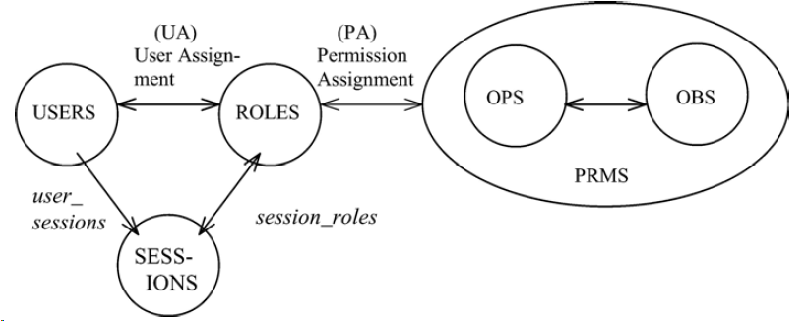
\includegraphics[width=4.0in]{sections/core-model.png}
    \caption{\label{fig:overview}Diagram in Core RBAC reference model\cite{ferraiolokuhn}.}
\end{figure}

Figure~\ref{fig:overview} presents an overview of core RBAC reference model diagram where entities and their relations are described.
Let "USERS", "ROLES", "OBS", "OPS", "PRM", and "SESSIONS" denote users, roles, objects, operations, permissions, and sessions, respectively.
Permissions are associated with possible users' pre-defined operation on an object (e.g., execute a file).
Note that, at user or role activation, a session associated with user or role is established.


\subsection{Hierarchical RBAC} 

The hierarchical RBAC Reference Model adds role hierarchies ($RH$) feature to the core RBAC Reference Model.
$RH$ incorporates a structure of roles in an organization using inheritance relationships among attributes such as roles.
The role structure in an organization may use
a role $r_1$, which inherits all permissions of another role $r_2$.
For example, a manager role may inherit all permissions of an employee role.
Role hierarchies help simplify access control policy creation and maintenance by reducing the number of
individual role assignments for a user. 
Concept of the role inheritance describes the many-to-many mapping role inheritance relations among roles.
Therefore, more than one role (e.g., two roles $r_1$ and $r_1'$) can inherit all permissions of $r_2$ 
General role hierarchies can be extended to use the concept of multiple inheritances where
$r_1$ inherits all permissions from more than one role (e.g., two roles $r_2$ and $r_2'$) .


\subsection{Constrained RBAC}

The constrained RBAC Reference Model incorporates separation of duty relations to  the core or the hierarchical RBAC Reference Model. Separation of 
duty relations enforces conflict of interest among roles. This model defines two types of separation of duty relations: static and dynamic.

\begin{itemize}
	\item Static Separation of Duty (SSoD): SSoD restricts the conflicting-roles, which can be assigned to a single user statically. Consider that roles $Role_A$ and $Role_B$ are conflicting with each other. On situations
	where multiple roles can be associated with a single user, no permission is given to a user who is assigned to both $Role_A$ and $Role_B$ statically. SSoD is known to be too rigid for practical use in cases where a user should have permissions when a user is assigned to both $Role_A$ and $Role_B$.
	For example, accounting clerk role requests a check and accounting manager role approves the check. These two roles must be
	mutually exclusive to avoid a situation where one approves the check that the one requested.
	
	\item Dynamic Separation of Duty (DSD): Dynamic SoD is known to be
more flexible than SSoD. DSD restricts the conflicting-role assignments dynamically that are associated with a user. Consider that roles $Role_A$ and $Role_B$ are conflicting with each other. For the situations where multiple roles can be associated with a single user, no permission is given to a user who is assigned to both $Role_A$ and $Role_B$ dynamically.	
Consider that one can be assigned to the accounting clerk and the accounting manager role at the same time.
In such a situation, DSD can enforce that the accounting manager role does not approve her/his requested checks but
approve only checks that others requested. This feature requires handling dynamic environments.
\end{itemize}
